\begin{figure}

    
    
      \tikzstyle{latent} = [circle,fill=white,draw=black,inner sep=1pt,
minimum size=30pt, font=\fontsize{15}{15}\selectfont, node distance=1]


  \newcommand{\ltkiz}{1cm}
  
  
\captionsetup[subfigure]{justification=centering}
    \centering  
    \begin{subfigure}[t]{0.3\textwidth}
        \centering   
		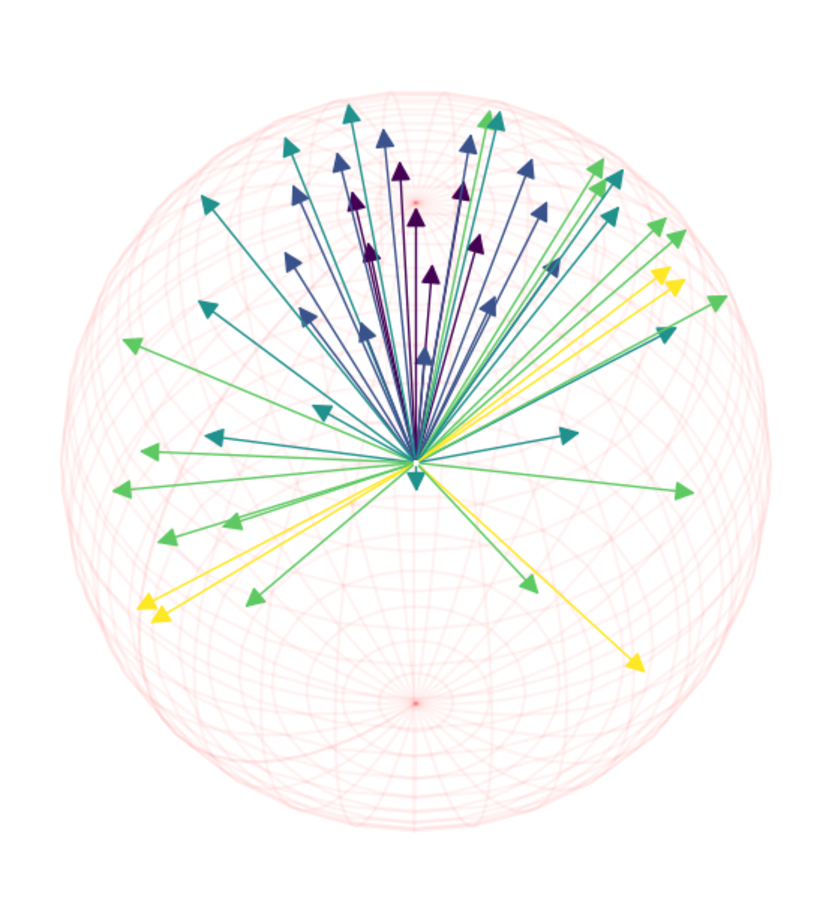
\includegraphics[width=3cm]{figures/angles.pdf}
        \caption{$s$: angle between the camera and the light source}
    \end{subfigure}%
    ~ 
    \begin{subfigure}[t]{0.3\textwidth}
        \centering  
		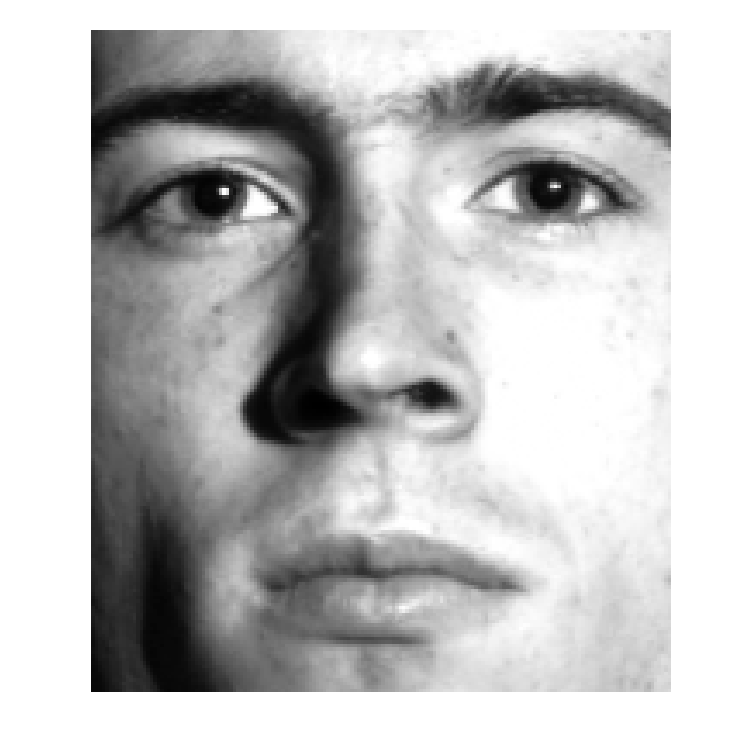
\includegraphics[width=0.7\textwidth]{figures/face.pdf}
        \caption{One image $x$ for a given lighting condition $s$ and person $y$}
    \end{subfigure}
        ~ 
    \begin{subfigure}[t]{0.3\textwidth}
        \centering  
        \scalebox{0.65}
        {
\tikz{ %
  \node[obs] (x) {${x}$} ; %
  \node[obs, above=0.5 * \ltkiz of x, xshift=+1.5\ltkiz] (s) {${s}$};
    \node[latent, above=0.5 * \ltkiz of x,xshift=0*\ltkiz] (z1) {${z_1}$};
      \node[obs, above=0.5 * \ltkiz of z1, xshift=+1.5\ltkiz] (y) {${y}$};
    \node[latent, above=0.5 * \ltkiz of z1,xshift=0*\ltkiz] (z2) {${z_2}$};    
    \edge {z1} {x};
    \edge{z2} {z1};
    \edge {y} {z1};
    \edge {s} {x};
} }
 \caption{Complete graphical model}
    \end{subfigure}
        \caption{Framework for learning invariant representations in the Extended Yale B Face dataset.}
    \label{hsicyale}
\end{figure}
